\chapter{Análise dos resultados}
\label{cht:analiseresultados}

Neste capitulo serão apresentadas algumas das observações e resultados obtidos ao longo dos diferentes cenários de construção e treino de RNAs para resolver o problema de classificação de testo. 

\begin{figure}[H]
    \hspace{-0.6in}
    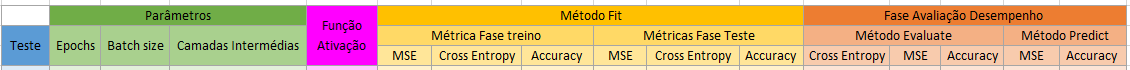
\includegraphics[scale=0.7]{Imagens/tabela.png}
    \caption{Informações registadas em cada cenários de teste e topologia de Rede exploradas}
    \label{fig:Tabela}
\end{figure}

O sumário dos resultados estará descrito através de uma tabela, caracterizada pelo formato visível na figura \ref{fig:Tabela} e que apresenta a seguinte estrutura:
\begin{itemize}[noitemsep]
    \item Cada coluna representa um parâmetro relevante no processo de treino ou teste da rede, como o número de \textit{Epochs}, \textit{Batch Size}, topologia da rede ou métricas de avaliação conseguidas; 

    \item Na coluna \textit{Camadas Intermédias}:
    \begin{itemize}[noitemsep]
        \item O número de camadas intermédias definidas é dado pelo comprimento do vetor;
        
        \item O número de nodos de cada camada, é dado pelo valor do índice \textit{i} que representa essa camada;
        
        \item Camadas de Dropout são identificadas pela letra \textit{D}. 
    \end{itemize}
    
    \item As \textit{Métricas da Fase Teste} dentro da opção \textit{Método Fit} (a amarelo) representam as avaliações nos cenários em que no método fit se utilizou o parâmetro \textit{Percentage split} com valor 0.33;
    
    \item A secção laranja, representa a avaliação do desempenho da rede, através dos métodos predict e evaluate disponibilizados na plataforma keras. 
    
    Em ambos as funções referidas é utilizado o mesmo dataset de teste, previamente criado e não utilizado em fase de treino. 
\end{itemize}

\newpage
\begin{figure}[H]
    \centering
    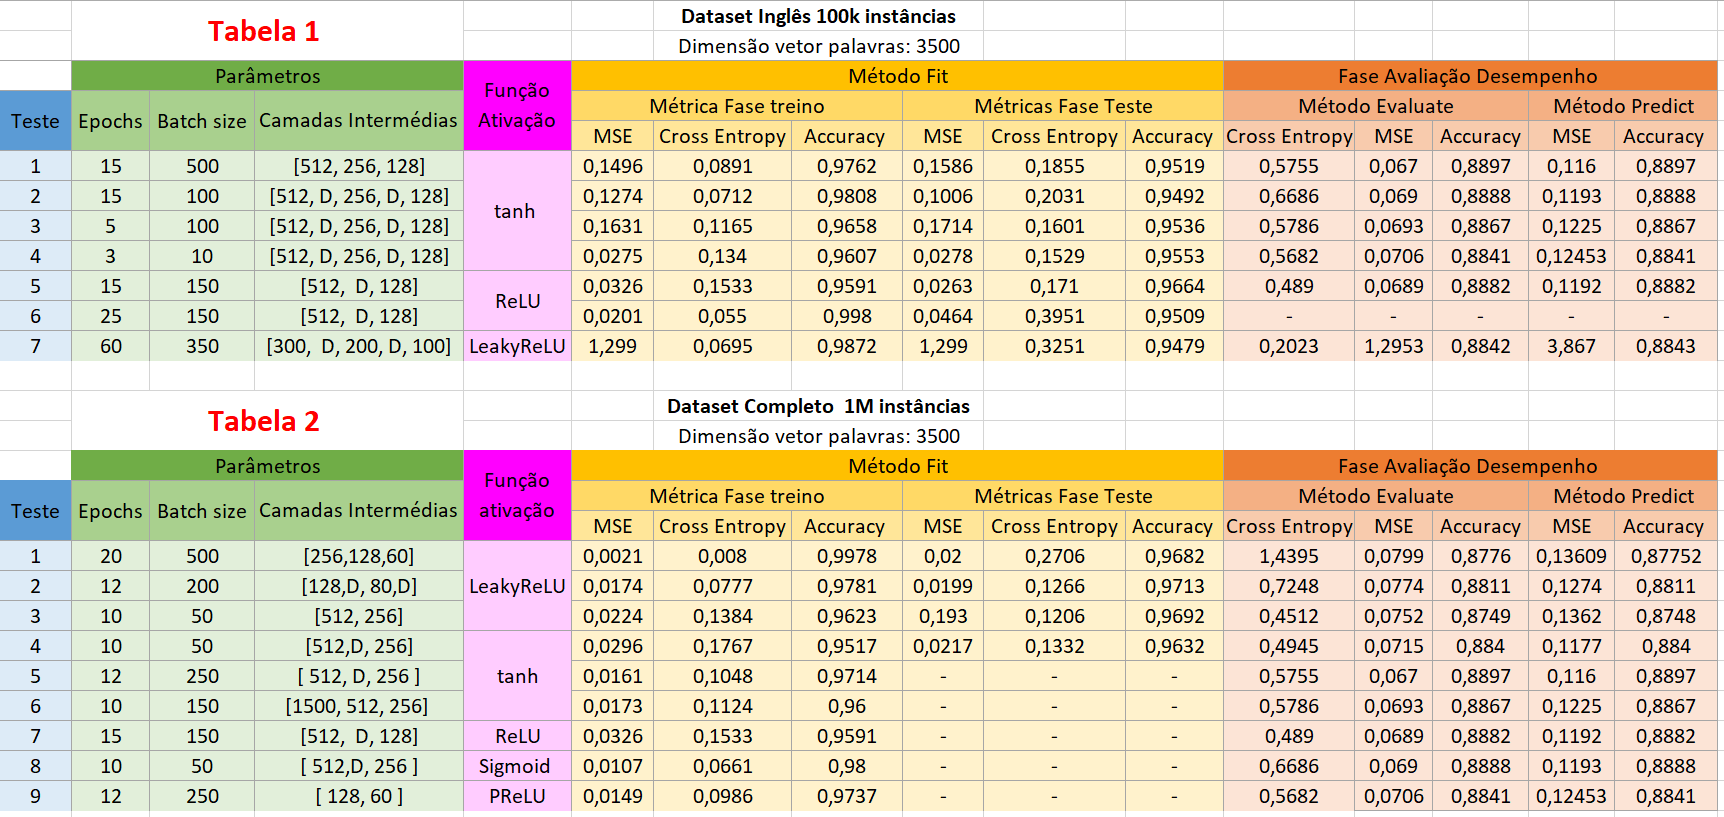
\includegraphics[scale=0.62, angle=90]{Imagens/tabelas.png}
    \caption{Tabelas com os parâmetros e resultados dos cenários de avaliação de desempenho das RNAs criadas.}
    \label{fig:tabelas}
\end{figure}

\section{Dataset completo \textit{Tweets}}

A Tabela 1 da Figura \ref{fig:tabelas} descreve os resultados os cenários de treino de RNAs realizados sobre a versão reduzida do dataset. 

Focando alguns dos resultados obtidos:
\begin{itemize}
    \item Numa primeira abordagem ao dataset completo, foram desde logo utilizadas algumas considerações destacadas nas secções \ref{sec:ParametrostreinoRede}.
    
    Para o Teste 1, foi inicialmente criada uma topologia de rede com 3 camadas intermédias, tendo cada uma delas, respetivamente, 256 e 128 e 60 neurónios. 
    
    Na tentativa de obter rapidamente bons resultados, utilizou-se como forma de inicialização dos pesos o método de \textit{Xavier} e como funções de ativação dos neurónios de cada camada selecionou-se a função LeakyReLU. 
    
    Foram realizadas 20 passagens pelos dados, alimentando a rede com 500 instâncias a cada iteração do treino. 
    
    \begin{figure}[H]
        \hspace{-0.4in}
        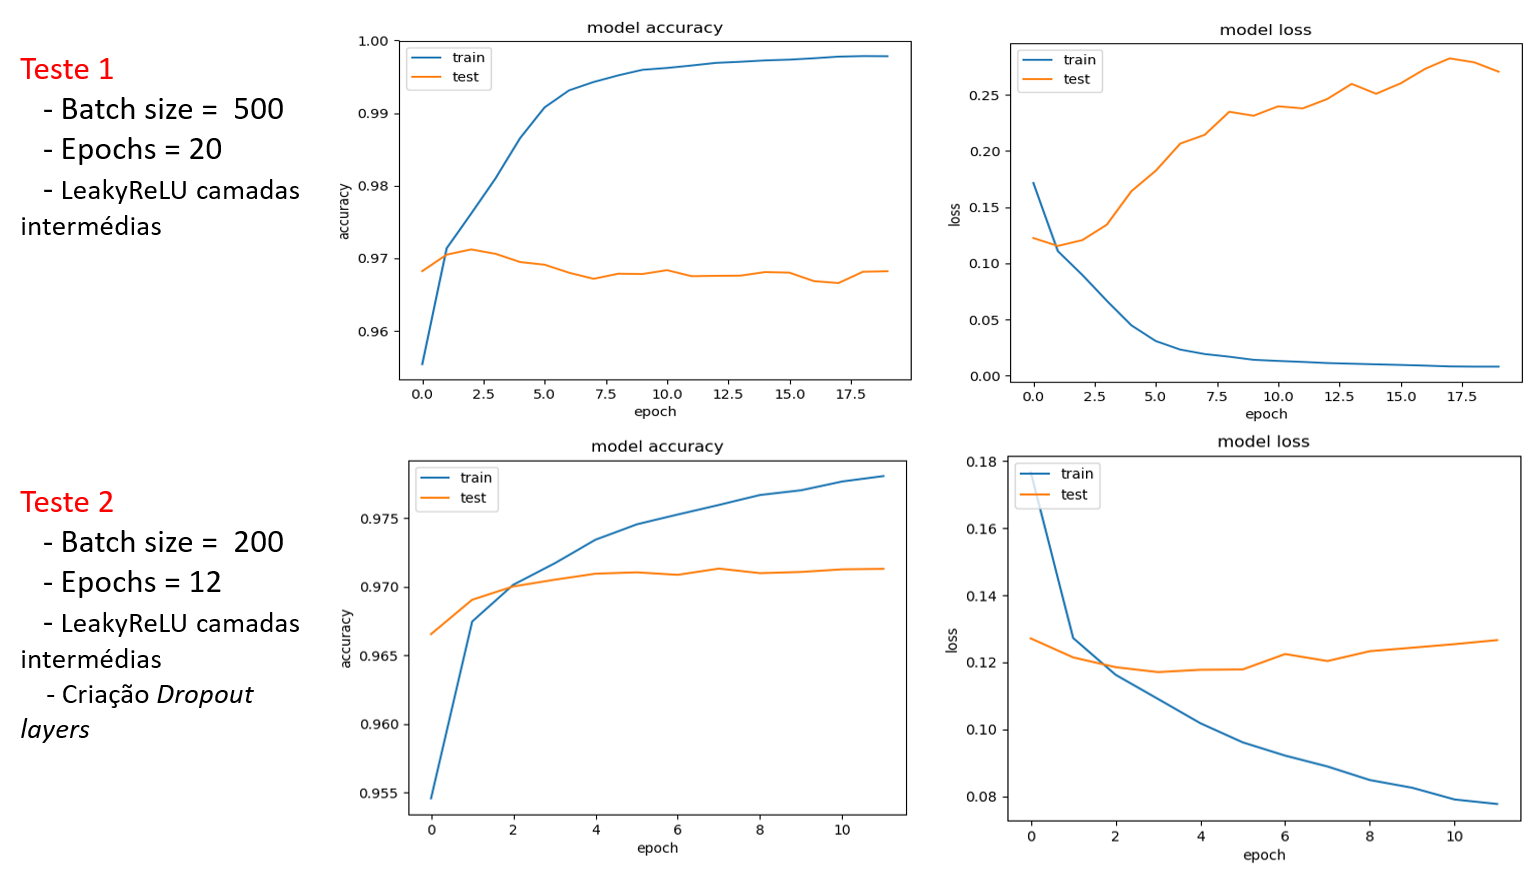
\includegraphics[scale=0.65]{Imagens/t37.png}
        \caption{Resultados Teste 1 e 2, com uso do dataset completo para criação de conjuntos de treino + teste.}
        \label{fig:teste1}
    \end{figure}
    
    Estes resultados (Figura \ref{fig:teste1}) tornam-se relevantes no sentido em que, apresentam desde logo um cenário de overfitting. A accuracy da rede no final da fase de treino apresenta-se na casa dos 99\% e, na fase de teste, atinge apenas os 88\%. 
    
    Na tentativa de reduzir este sobre ajustamento aos dados, no Teste 2 procurou-se introduzir camadas de \textit{Dropout} na rede e simplificar a sua complexidade, reduzindo a topologia para duas camadas com, respetivamente, 128 e 80 nodos. 
    
    Apesar destas alterações reduzirem o valor de \textit{accuracy} em fase de treino, o valor de 97\% continua relativamente superior face aos 88\% novamente obtidos na fase de teste. 
    
    \item Independente da função de ativação utilizada nas camadas intermédias da rede, mesmo que o seu contradomínio não se apresente entre [-1, 1], como no caso da ReLU ou da Sigmoide, foi mesmo assim possível obter uma taxa de acertos de cerca de 88\% em fase de Teste da RNA. 
    (Relembrando que o output deve ser -1, 0 ou 1, conforme a classificação de um texto num sentimento negativo, neutro ou positivo) 
    
    Estes resultados permitem observar que as camadas intermédias são capazes de generalizar a informação que analisam, mesmo que não propaguem entre si sinais com valores negativos. 
    
    Ao longo das iterações de treino, as sinapses das camadas intermédias com estas funções ReLU ou Sigmoide não transmitem valores negativos, porque o seu contradomínio é positivo. Contudo, o peso das ligações (\textit{W}) pode eventualmente ajustar-se para valores negativos, sendo assim capazes de influenciar a aprendizagem da rede a ajustar-se inevitavelmente aos dados. 
    
    \item Relativamente ao Teste 7, foi utilizada uma topologia de rede com 3 camadas intermédias, possuindo 300, 200 e 100 neurónios, respetivamente. 
    Foi também a inicialização dos pesos com o método de \textit{Xavier} e utilizada a função LeakyReLU.  
    
    \begin{figure}[H]
        \hspace{-0.4in}
        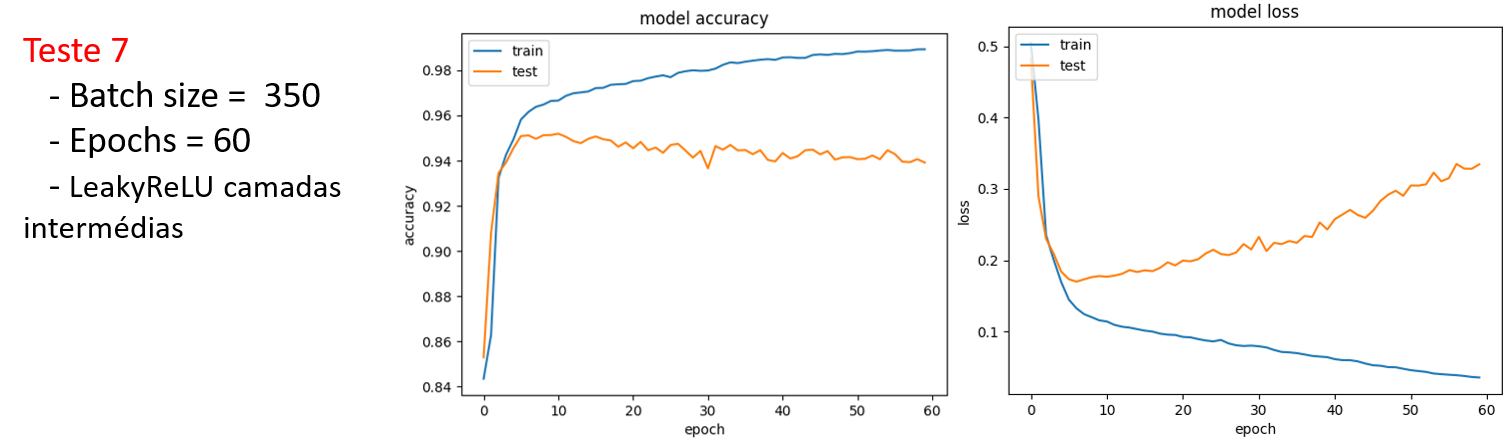
\includegraphics[scale=0.65]{Imagens/t7.png}
        \caption{Resultados do Teste 7, com uso do dataset completo para criação de conjuntos de treino + teste.}
        \label{fig:teste4}
    \end{figure}
    
    A análise dos resultados conseguidos com esta arquitetura e apresentados na Figura \ref{fig:teste4} é interessante devido à evolução das curvas a cada \textit{Epochs}. 
    
    O surgimento de picos (altos e baixos em \textit{accuracy}) ao longo das diferentes \textit{Epochs} permite concluir que com estas configurações, a função de ativação ou as métricas de avaliação não são as mais indicadas. 
    Isto porque, num determinado \textit{Epoch}, a atualização dos gradientes através da métrica \textit{Loss} definida leva a bons resultados mas, num \textit{Epochs} seguinte, os resultados já não são favoráveis. 
    
    \item No geral, independente da topologia ou parâmetros utilizados, os valores de accuracy em fase de teste, com dados exclusivamente reservados para treino, rondam sempre os 88\%. 
\end{itemize}
    

\section{Dataset \textit{Tweets} em Inglês}

A Tabela 2 da Figura \ref{fig:tabelas} descreve os resultados os cenários de treino de RNAs realizados sobre a versão reduzida do dataset e segue a mesma estrutura descrita na secção anterior.

Relembrando, este conjunto de dados contem apenas publicações em inglês e, por apresentar menores dimensões, permite explorar vetores de palavras com maiores dimensões e redes com maior complexidade, pois dá mais folga a nível dos recursos de memória necessários para o analisar.

Apenas descrevendo alguns dos principais resultados obtidos: 

\begin{itemize}
    \item Numa primeira abordagem (Teste 1 e 2), foi utilizada uma topologia de rede com 3 camadas intermédias, tendo cada uma delas, respetivamente, 512, 256 e 128 neurónios. 

    Como funções de ativação utilizou-se a função tangente hiperbólica \textit{tanh} e os pesos das ligações foram inicializados com uma distribuição uniforme. 
    
    \begin{figure}[H]
        \hspace{-0.4in}
        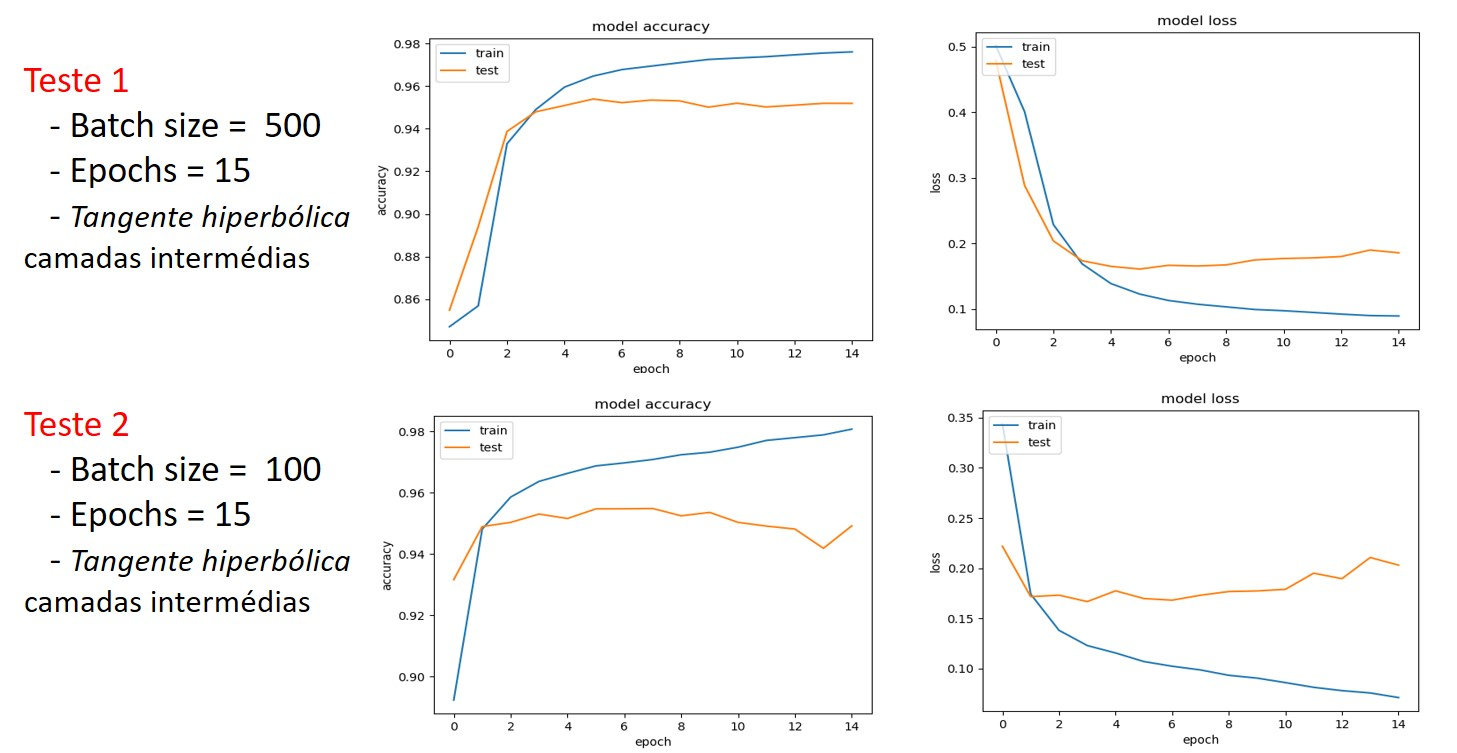
\includegraphics[scale=0.67]{Imagens/teste1.jpg}
        \caption{Resultados Teste 1 e Teste 2 com o dataset reduzido apenas com publicações em inglês}
        \label{fig:teste2}
    \end{figure}
    
    Observando os gráficos da Figura \ref{fig:teste2}, as retas descreverem inicialmente um cenário de overfitting, onde os valores de \textit{accuracy e cross entrophy (loss)} na fase de treino se apresentam ligeiramente superiores face à fase de avaliação de desempenho. 

    No Teste 2, realizar um teste com o mesmo número de \textit{epochs} (15) mas reduzindo o parâmetro \textit{batch size} de 500 para 100 exemplos contribuiu apenas para acentuar ligeiramente os resultados de \textit{overfitting} já assinalados. 
    
    O crescimento suave da curva de \textit{accuracy} na fase de treino, permite assumir que a função de ativação e avaliação internas da rede levam a um correto ajustamento dos pesos a cada iteração, permitindo assim uma aprendizagem gradual, sem grandes variações entre cada \textit{Epoch}.
    
    \item Reduzir o número de \textit{Epochs} para um valor abaixo das dezenas (Teste 3 e Teste 4) não permite nenhuma avaliação concreta ao desempenho de aprendizagem da rede. 
    As informações dos gráficos nestes cenários não são suficientes para compreender a evolução da rede na fase de treino. 
    
    Contudo, as métricas devolvidas foram registadas e enquadram-se dentro dos resultados dos restantes testes. 
    
   \item Relativamente ao Teste 6, foi aumentado o número de \textit{Epochs}, procurando tirar o melhor partido possível da função de ativação \textit{ReLU}. 
   
   Contudo, o maior número de \textit{Epochs} permitiu apenas aumentar o efeito de \textit{overfitting} já visualizado noutros cenários de treino. A accuracy a nivel de treino manteve-se próxima dos 88\%.
   
   \begin{figure}[H]
        \hspace{-0.4in}
        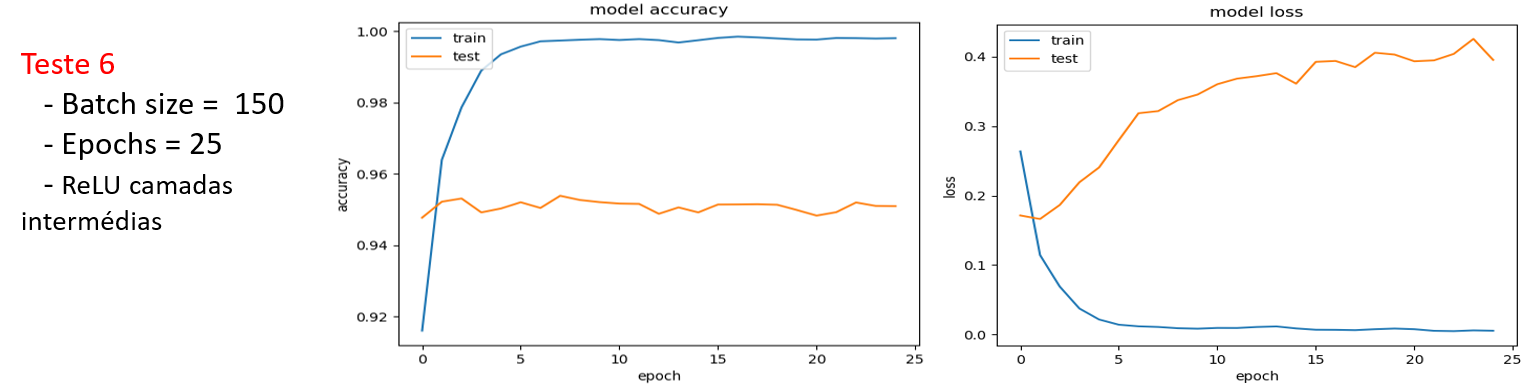
\includegraphics[scale=0.65]{Imagens/t2.png}
        \caption{Resultados Teste 6, com o  dataset reduzido apenas com publicações em inglês}
        \label{fig:teste3}
    \end{figure}
   
\end{itemize}